In this section, we present the fundamental ideas that form the basis of the developed approach. Subsection \ref{AA:Welford} explains Welford's online algorithm, which can adjust distribution to changes in real-time. Subsection \ref{AA:InvWelford} proposes a two-pass implementation that can reverse the impact of expired samples. The math behind distribution modeling in Subsection \ref{AA:Distribution} establishes the foundation for the Gaussian anomaly detection model discussed in Subsection \ref{AA:Anomaly}, followed by conditional probability computation in Subsection \ref{AA:Conditional}. The last subsection of the preliminaries is devoted to the definition of anomalies.

\subsection{Welford's Online Algorithm}\label{AA:Welford}
Welford introduced a numerically stable online algorithm for calculating mean and variance in a single pass through data. Therefore, the algorithm allows the processing of IoT device measurements without the need to store their values \citep{Wel62}.

Given measurement \(x_i\) where \(i=1,...,n\) is a sample index in sample population \(n\), the corrected sum of squares \(S_n\) is defined as
\begin{equation}
S_n = \sum_{i=1}^n (x_i - \bar x_n)^2\text{,}\label{eq:sumsquares}
\end{equation}
with the running mean \(\bar x_n\) defined as previous mean \(\bar x_{n-1}\) weighted by proportion of previously seen population \(n-1\) corrected by current sample as
\begin{equation}
\bar x_n = \frac{n-1}{n} \bar x_{n-1} + \frac{1}{n}x_n = \bar x_{n-1} + \frac{x_n - \bar x_{n-1}}{n}\text{.}\label{eq:runmean}
\end{equation}
Throughout this paper, we consider the following formulation of an update to the corrected sum of squares:
\begin{equation}
S_n = S_{n-1} + (x_n - \bar x_{n-1})(x_n - \bar x_n)\text{,}\label{eq:upsumsquares}
\end{equation}
as it is less prone to numerical instability due to catastrophic cancellation, significant loss of precision due to subtracting two nearly equal numbers. Finally, the corresponding unbiased variance is
\begin{equation}
s^2_n = \frac{S_{n}}{n-1}\text{.}\label{eq:runvar}
\end{equation}

This implementation of the Welford method requires the storage of three scalars: \(\bar x_{n-1}\); \(n\); \(S_n\).

\subsection{Inverting Welford's Algorithm}\label{AA:InvWelford}
Based on \eqref{eq:runmean}, it is clear that the influence of the latest sample over the running mean decreases as the population \(n\) grows. For this reason, regulating the number of samples used for sample mean and variance computation has crucial importance over adaptation. Given access to the instances used for computation and expiration period \(\ui{t}{e} \in \mathbb{N}_{0}^{n-1}\), reverting the impact of \(x_{n-\ui{t}{e}}\) can be written as follows

\begin{equation}
S_{n-1} = S_n - (x_{n-\ui{t}{e}} - \bar x_{n-1})(x_{n-\ui{t}{e}} - \bar x_n)\text{,}\label{eq:revrunmean}
\end{equation}

where the reverted mean is given as

\begin{equation}
\bar x_{n-1} = \frac{n}{n-1} \bar x_{n} - \frac{1}{n-1}x_{n-\ui{t}{e}} = \bar x_{n} - \frac{x_{n-\ui{t}{e}} - \bar x_{n}}{n-1}\text{.}\label{eq:revmean}
\end{equation}


Finally, the unbiased variance follows the formula:

\begin{equation}
s^2_{n-1} = \frac{S_{n-1}}{n-2}\text{.}\label{eq:revvar}
\end{equation}

Notably, inversion allows the algorithm to keep a constant rate of adaptation at the cost of storing a bounded data buffer.

\subsection{Statistical Model of Multivariate System}\label{AA:Distribution}
Multivariate normal distribution generalizes the multivariate systems to the model where the degree to which variables are related is represented by the covariance matrix. Gaussian normal distribution of variables is a reasonable assumption for process measurements, as it is a common distribution that arises from stable physical processes measured with noise \citep{Mishra201831}. The general notation of multivariate normal distribution is:
\begin{equation}
 \mathbf{X}\ \sim\ \mathcal{N}_k(\boldsymbol\mu,\, \boldsymbol\Sigma)\text{,}\label{eq:distribution}
\end{equation}

where $k$-dimensional mean vector is denoted as \(\boldsymbol\mu = (\bar x_{1},...,\bar x_{k})^T\ \in \mathbb{R}^{k}\) and \(\boldsymbol\Sigma \in \mathbb{R}^{k\times{k}}\) is the $k \times k$ covariance matrix, where \(k\) is the index of last random variable.

The probability density function (PDF) \(f(\boldsymbol{x}; \boldsymbol{\mu}, \boldsymbol{\Sigma})\) of multivariate normal distribution is denoted as:
\begin{equation}
f(\boldsymbol{x}; \boldsymbol{\mu}, \boldsymbol{\Sigma}) = \frac{1}{(2\pi)^{k/2} |\boldsymbol{\Sigma}|^{1/2}} e^{-\frac{1}{2} (\boldsymbol{x}-\boldsymbol{\mu})^\top \boldsymbol{\Sigma}^{-1} (\boldsymbol{x}-\boldsymbol{\mu})}\text{,}
\end{equation}

where $\boldsymbol{x}$ is a $k$-dimensional vector of measurements $x_i$ at time $i$, $|\boldsymbol{\Sigma}|$ denotes the determinant of $\boldsymbol{\Sigma}$, and $\boldsymbol{\Sigma}^{-1}$ is the inverse of $\boldsymbol{\Sigma}$.

The cumulative distribution function (CDF) of a multivariate Gaussian distribution describes the probability that all components of the random vector \(\boldsymbol{X}\) take on a value less than or equal to a particular point \(q\) in space, and can be used to evaluate the likelihood of observing a particular set of measurements or data points. In other words, it gives the probability of observing a random vector that falls within a certain region of space. The standard notation of CDF is as follows:

\begin{equation}
F(\boldsymbol{x}; \boldsymbol{\mu}, \boldsymbol{\Sigma}) = \int_{-\infty}^{q} f(\boldsymbol{x}; \boldsymbol{\mu}, \boldsymbol{\Sigma}) \text{d}\boldsymbol{x}\text{,}\label{eq:cdf}
\end{equation}

where $\text{d}\boldsymbol{x}$ denotes the integration over all $k$ dimensions of $\boldsymbol{x}$.

As the equation \eqref{eq:cdf} cannot be integrated explicitly, an algorithm for numerical computation was proposed in \citet{Genz2000}.

Given the PDF, we can also determine the value of \(\boldsymbol{x}\) that corresponds to a given quantile $q$ using a numerical method for inversion of CDF (ICDF) often denoted as percent point function (PPF) or $F(\boldsymbol{x}; \boldsymbol{\mu}, \boldsymbol{\Sigma})^{-1}$. An algorithm that calculates the value of the PPF is part of standard statistical software tools.

\subsection{Conditional Probability Distribution}\label{AA:Conditional}
% https://statproofbook.github.io/P/mvn-cond.html
% @misc{https://doi.org/10.5281/zenodo.4305950,
% doi = {10.5281/ZENODO.4305950},
% url = {https://zenodo.org/record/4305950},
% author = {Soch, Joram and Proofs, The Book Of Statistical and Faulkenberry, Thomas J. and Petrykowski, Kenneth and Allefeld, Carsten},
% title = {StatProofBook/StatProofBook.github.io: StatProofBook 2020},
% publisher = {Zenodo},
% year = {2020},
% copyright = {Open Access}
% }
Considering that we observe particular vector $\boldsymbol{x}_i$, we can update probability distributions, calculated according to the rules of conditional probability, of individual measurements within the vector given the rest of the measurements in $\boldsymbol{x_{i}}$.
Let's assume multivariate normal distribution \eqref{eq:distribution} and without loss of generality, that the vector $\boldsymbol{x}_i$ can be partitioned into subset variable $x_a$, and complement vector $\boldsymbol{x_b}$ as follows

\begin{equation}
 \boldsymbol{x}_i = \begin{bmatrix}x_a \\ \boldsymbol{x_b} \end{bmatrix} \text{with dimensions} \begin{bmatrix}1\times 1 \\ (k - 1) \times 1\end{bmatrix} \text{,}
\end{equation}

where $a = 1,...,k$ and $\boldsymbol{b} = \{1, 2, \ldots, k\} \text{ where }a \notin \boldsymbol{b}$. This partitioning allows us to define block-wise mean and covariance as follows:

\begin{equation}
 \boldsymbol\mu = \begin{bmatrix}\mu_a \\ \boldsymbol{\mu_b} \end{bmatrix} \text{with dimensions} \begin{bmatrix}1\times 1 \\ (k - 1) \times 1\end{bmatrix} \text{,}
\end{equation}
and
\begin{equation}
 \boldsymbol\Sigma = \begin{bmatrix}\sigma_{aa}^2 & \boldsymbol\Sigma_{a\boldsymbol{b}} \\ \boldsymbol\Sigma_{\boldsymbol{b}a} & \boldsymbol\Sigma_{\boldsymbol{bb}} \end{bmatrix}
 \text{with dimensions} \begin{bmatrix}1\times 1 & 1\times (k - 1) \\ (k - 1) \times 1 & (k - 1) \times (k - 1)\end{bmatrix} \text{.} \label{eq:sigma}
\end{equation}

Subsequently, we can derive the conditional distribution of any subset variable $x_a$, given the complementary vector $\boldsymbol{x_b}$. This conditional distribution conforms to a univariate normal distribution, characterized by:

\begin{equation}
  X_a \mid \mathbf{X}_{\boldsymbol{b}} \sim\ \mathcal{N}(\mu_{a \mid \boldsymbol{b}},\, \sigma_{a \mid \boldsymbol{b}}^2)\text{.}\label{eq:cond_distribution}
\end{equation}

where $\mu_{a \mid \boldsymbol{b}}$ denotes the conditional mean and $\sigma_{a \mid \boldsymbol{b}}^2$ represents the conditional variance. These crucial parameters can be computed by applying the Schur complement as follows:

\begin{equation}
  \sigma_{a \mid \boldsymbol{b}}^2 = \sigma_{aa}^2 - \boldsymbol\Sigma_{a\boldsymbol{b}} \boldsymbol\Sigma_{\boldsymbol{bb}}^{-1} \boldsymbol\Sigma_{\boldsymbol{b}a}\text{,}\label{eq:cond_var}
\end{equation}

for the conditional variance $\sigma_{a \mid \boldsymbol{b}}^2$, while the conditional mean, denoted as $\mu_{a \mid \boldsymbol{b}}$, is determined by:

\begin{equation}
  \mu_{a \mid \boldsymbol{b}} = \mu_a + \boldsymbol\Sigma_{a\boldsymbol{b}} \boldsymbol\Sigma_{\boldsymbol{bb}}^{-1} (\boldsymbol{x_b} - \boldsymbol\mu_b)\text{.}\label{eq:cond_mean}
\end{equation}

The conditional variance $\sigma_{a \mid \boldsymbol{b}}^2$ essentially represents the Schur complement of $\boldsymbol\Sigma_{\boldsymbol{bb}}$ within the overall covariance matrix $\boldsymbol\Sigma$.

\subsection{Gaussian Anomaly Detection}\label{AA:Anomaly}
From a viewpoint of statistics, outliers are commonly denoted as values that significantly deviate from the mean. Under the assumption that the spatial and temporal characteristics of a system, observed over a moving window, can be suitably represented as normally distributed features, we assert that any anomaly can be identified as an outlier.

In empirical fields like machine learning, the three-sigma rule ($3\sigma$) provides a framework for characterizing the region of a distribution within which normal values are expected to fall with high confidence. This rule renders approximately 0.265\% of values in the distribution as anomalous.

The \(3\sigma\) rule establishes the probability that any sample \(x_a\) of a random vector \({X}\) falls within a given CDF over a semi-closed interval as the distance from the conditional mean \(\mu_{a \mid \boldsymbol{b}} \) of 3 conditional variances \(\sigma_{a \mid \boldsymbol{b}}^2\) and gives an approximate value of $q$ as
\begin{equation}
q=P\{|x_a-\mu_{a \mid \boldsymbol{b}} |<3\sigma_{a \mid \boldsymbol{b}}^2\}=0.99735
\text{.}\label{eq:q}
\end{equation}

Utilizing a probabilistic model of normal behavior, we can determine threshold values ${\ui{x}{l}}$ and ${\ui{x}{u}}$ corresponding to the closed interval of the CDF where this probability is established. The inversion of Equation \eqref{eq:cdf} facilitates this calculation, yielding:

\begin{equation}
{\ui{x}{l}} = F((1 - P\{|x_a-\mu_{a \mid \boldsymbol{b}}|<3\sigma_{a \mid \boldsymbol{b}}^2\}); \mu_{a \mid \boldsymbol{b}}, \sigma_{a \mid \boldsymbol{b}}^2)^{-1}\text{,}\label{eq:thresh_low}
\end{equation}

for the lower limit, and

\begin{equation}
{\ui{x}{u}} = F((P\{|x_a-\mu_{a \mid \boldsymbol{b}}|<3\sigma_{a \mid \boldsymbol{b}}^2\}); \mu_{a \mid \boldsymbol{b}}, \sigma_{a \mid \boldsymbol{b}}^2)^{-1}\text{,}\label{eq:thresh_high}
\end{equation}

for the upper limit. These lower and upper limits together form vectors $\boldsymbol{\ui{x}{l}}$ and $\boldsymbol{\ui{x}{u}}$, respectively, defining the region of normal system operation. This region is conceptualized as a hypercube in the feature space, with each dimension bounded by the corresponding feature limits, as computed using Equations \eqref{eq:thresh_low} and \eqref{eq:thresh_high} for all $a = 1,...,k;~ \boldsymbol{b} = \{1, 2, \ldots, k\}$ where $a \notin \boldsymbol{b}$. The approximation of a confidence ellipse as a hypercube can be employed to represent the region of normal system operation for individual variables of a multivariate system, rendering it as an aid for visual representation.

The predicted state of the system, denoted as $y_i$, and the normality of signals $\uis{\boldsymbol{y}}{s}{i}$ at time $i$ are determined based on the maximum distance of observations from the center of the probabilistic density. The center of the probabilistic density corresponds to the vector of conditional means $\mu_{a \mid \boldsymbol{b}}$ with respect to other features. The calculation of this distance involves the cumulative distribution function (CDF) of observations and conditional distributions, as  follows:

% https://stats.stackexchange.com/questions/186402/expressing-conditional-covariance-matrix-in-terms-of-covariance-matrix

\begin{equation}
 {F(x_a; \mu_{a \mid \boldsymbol{b}}, \sigma_{a \mid \boldsymbol{b}}^2)}:a = 1,...,k;~ \boldsymbol{b} = \{1, 2, \ldots, k\} \text{ where }a \notin \boldsymbol{b} \text{.}\label{eq:max_score}
\end{equation}

Subsequently, operation states of individual inputs are defined as follows:

\begin{equation}
 \uis{\boldsymbol{y}}{s}{i} =
 \begin{cases}
 0 & \text{ if } T \leq \eqref{eq:max_score}
 \\
 1 & \text{ if } T > \eqref{eq:max_score}
 \text{,}\label{eq:anomaly_signal}
 \end{cases}
\end{equation}

where $T$ represents a threshold that distinguishes between normal signal measurement ($\uis{\boldsymbol{y}}{s}{i} = 0$) and abnormal ($\uis{\boldsymbol{y}}{s}{i} = 1$).

For the overall abnormality of the system, any anomaly in signals $\uis{\boldsymbol{y}}{s}{i}$ is considered, resulting in:

\begin{equation}
 y_i =
 \begin{cases}
 1 & \text{if } 1 \in \uis{\boldsymbol{y}}{s}{i}
 \\
 0 & \text{otherwise}
 \text{,}\label{eq:anomaly}
 \end{cases}
\end{equation}


defining the discrimination boundary between system operation where $y_i = 0$ indicates normal system operation, and $y_i = 1$ indicates anomalous operation.

\subsection{Anomaly Definition}\label{AA:AnomalyDefinition}
This subsection provides an overview of the definition of anomalies in data analysis and their categorization, setting conventions for this paper.

In the realm of data analysis, anomalies are conspicuous deviations from the anticipated patterns within a dataset. Traditionally, the task of anomaly detection has relied upon unsupervised methodologies, wherein the identification of "outliers" entails the comparison of data points in both temporal and spatial contexts. This approach, often referred to as point-wise anomaly detection, classifies a data point as an anomaly when it exhibits significant dissimilarity from its neighboring data points \citep{IGLESIASVAZQUEZ2023120994}.

The concept of point anomalies, influenced by factors such as temporal and spatial aspects, can be further categorized into conditional and contextual anomalies \citep{Ruff2021}.

Nevertheless, this conventional method may not be suitable for scenarios characterized by collective anomalies, where clusters of abnormal data points coexist. A more pragmatic approach defines anomalies as deviations from established "normal" patterns, resembling the principles of semi-supervised learning. Change point detection, in a similar vein, can be regarded as a relative approach that takes into account the varying dynamics of changes, whether they occur gradually or abruptly \citep{IGLESIASVAZQUEZ2023120994}.

It is imperative to recognize that the interpretation of anomalies, outliers, and novelties can vary upon the application. Anomalies typically garner significant attention, while outliers are often treated as undesirable noise and are typically excluded during data preprocessing. Novelties, on the other hand, signify new observations that necessitate model updates to adapt to an evolving environment \citep{Ruff2021}.

Notwithstanding the differences in terminology, methods employed for the identification of data points residing in low-probability regions, irrespective of whether they are referred to as "anomaly detection," "outlier detection," or "novelty detection," share fundamental similarities \citep{IGLESIASVAZQUEZ2023120994}.

\added{For visual clarity, Figure \ref{fig:anomaly} illustrates the differences between point anomalies, collective anomalies, and change points.}

\begin{figure}[htbp]
  \centering
  \resizebox{\linewidth}{!}{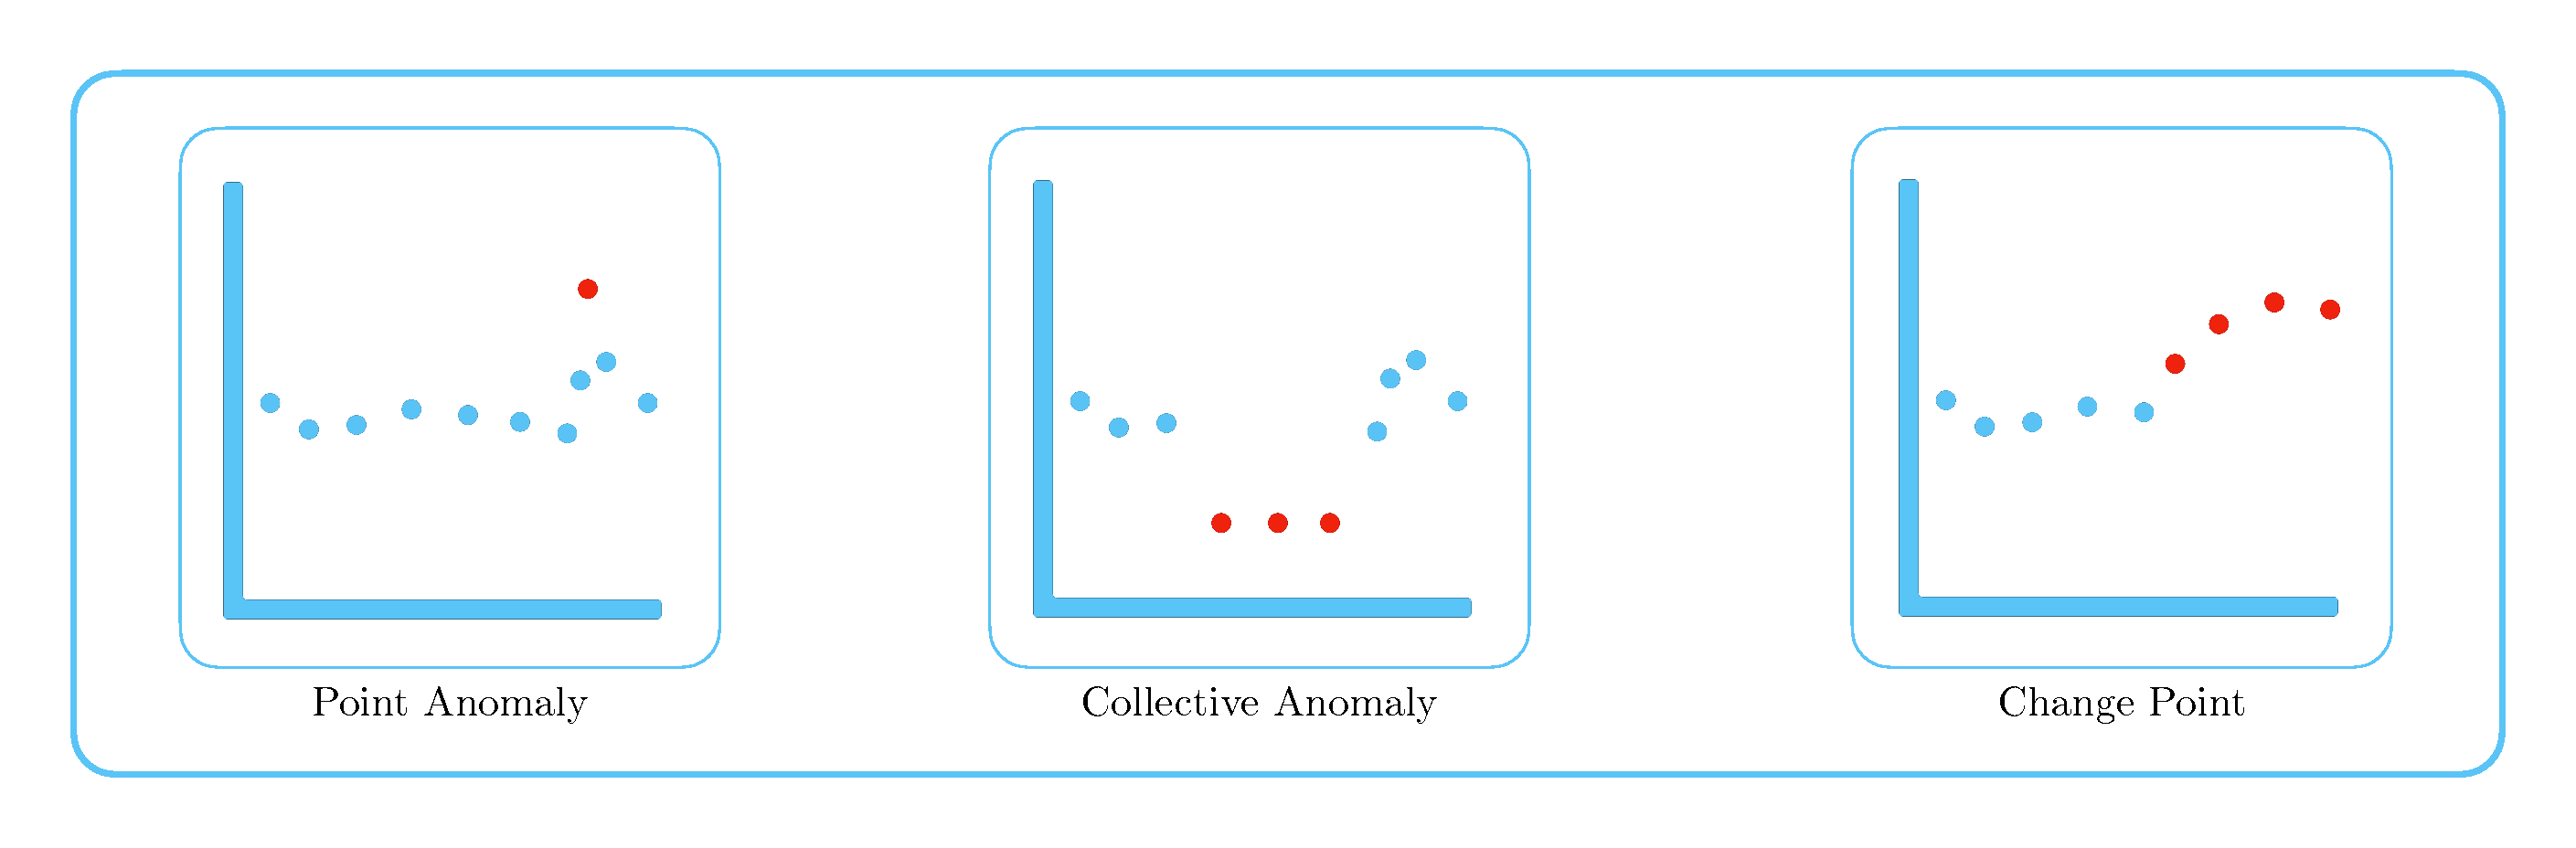
\includegraphics{figures/anomaly_definition.pdf}}
  \caption{\added{Ilustration of point anomaly, collective anomaly, and change point.}}
  \label{fig:anomaly}
\end{figure}